\chapter{Evaluation and Results} \label{chap:evaluation}


\begin{verbatim}
- no publicly available benchmarks for 360\degree image synthesis / image based rendering available for comparison with other methods
- scope: basic evaluation of mathematically measurable values (no human perception)
- create virtual datasets to test the limits of the method
- capture real datasets to perform a proof of concept

- these datasets could be used in the future to compare different algorithms
- benchmark used will be nearest neighbor (naive algorithm)
\end{verbatim}

\section{Evaluation Methodology}
\subsection{Approach}
\subsection{Error Calculation}
In order to evaluate the synthesized images, it is necessary to define a metric with which to measure their accuracy. Since it is outside of the scope of this thesis to evaluate human perception of the quality of the results, different error metrics are used to compare each result to its ground truth image. Two different metrics are used that measure different image features so that potential limitations of each metric can be compensated for.

\paragraph{L1 error on RGB}
The first metric is the L1 error calculated on the ground truth and result images in RGB color space. This is a simple error metric that calculates the mean absolute difference of the RGB values. The RGB differences are added together for the complete image and then divided by the number of pixels in the image. This results in an error value $e \in [0,3]$, since the maximum error per pixel is 3 for color values $RGB \in [0,1]$. The L1 error can also be visualized by calculating the absolute difference per pixel without averaging the values. Figure~\ref{fig:l1_example} shows an example visualization of the L1 error between two images. The visualization encodes areas of the image where there is a very large difference with a value closer to white and areas where there is no difference as black, which clearly shows where the problematic areas are in the image. \todo{why L1}

\begin{figure}
\centering
    \hfill
    \begin{subfigure}[t]{0.3\textwidth}
            \centering
            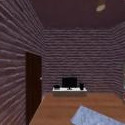
\includegraphics[width=0.9\textwidth]{04/l1_ex01.jpg}
            \caption{}
    \end{subfigure}%
    \hfill
    \begin{subfigure}[t]{0.3\textwidth}
            \centering
            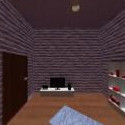
\includegraphics[width=0.9\textwidth]{04/l1_ex02.jpg}
            \caption{}
    \end{subfigure}
    \hfill
    \begin{subfigure}[t]{0.3\textwidth}
            \centering
            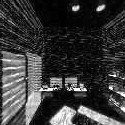
\includegraphics[width=0.9\textwidth]{04/l1_ex03.jpg}
            \caption{L1 error visualization of (a) and (b)}
    \end{subfigure}%
    \hfill
    \hfill
  \caption[Example visualization of L1 RGB error]{Example visualization of L1 RGB error. The RGB error values have been intensified so that they are more visible.} \label{fig:l1_example}
\end{figure}

As in the case of optical flow calculation, some adjustment must be made to adapt this metric for 360\degree images. Since the equirectangular projection is not equal-area, the areas towards the poles would intrinsically have higher weighting, since RGB L1 is calculated per pixel. In order to avoid this problem, the cube map projection is used, since it does not significantly distort the image. The average value is then calculated using the six faces of the cube, omitting the black background.

\paragraph{SSIM error on Grayscale}
The other metric to complement the RGB L1 error uses the structural similarity index (SSIM) \cite{ssim}, which measures the \emph{similarity} between two images. Instead of comparing the images pixel by pixel, the SSIM uses the luminance, contrast and structure of the images for comparison. Instead of comparing these features globally, it compares them locally, i.e.\ it compares smaller areas instead of the image as a whole. As a result, it is possible that the SSIM does not register small displacements in the scene if the objects are not distorted. However, the additional comparison with the RGB L1 error should mitigate this potential problem.

The SSIM metric in general, and the implementation used in the evaluation return a value $\in [-1, 1]$ with 1 signifying an extremely similar image and -1 signifying a very different image. In order to more easily compare it with the RGB L1 error, the SSIM value is converted to an error value $ e \in [0,1]$, with 0 signifying an identical image and 1 signifying a very different image.

The SSIM error is calculated on the grayscale image in cubemap representation. There is no need to use an RGB image, since it does not use the color values of an image. The cubemap representation is again used for its minimal distortion attribute, since the behavior of the SSIM on distorted images is not clear.

\subsection{Result Visualization}
- compare complete scenes with boxplot
- compare positions in the scene with top view + color coded viewpoints
- qualitative examination of specific result images

\section{Evaluation of Limits using Virtual Scenes}

\subsection{Parameters}
internal vs external parameters
\begin{itemize}
  \item internal:
  \item viewpoint density
  \item distance of scene from model (checkersphere, square room, arbitrary room)
  \item choice of gt points \ar fixed
  \item flow-based blending vs deviation-angle-based blending
  \item external:
  \item number of samples/viewpoints used for interpolation \ar two vs all within semi-large radius (all would be very computation intensive)
  \item limit to certain scenarios so that the explored space stays manageable
\end{itemize}

\subsubsection{Choice of Ground Truth Viewpoints and Captures}

\subsubsection{Selection of Input Viewpoints}

\subsubsection{Scene Distance from Model Sphere}
Checkersphere, square room, oblong room, (oblong room v2)

\subsection{Synthesizing Ground Truth Optical Flow}
 only makes sense to compare if flow algorithm works more or less correctly \ar narrows the parameter space for comparison
\begin{itemize}
  \item optical flow ground truth is impossible to get from real scenes
  \item however, virtual scenes contain all necessary information for retrieving ground truth for optical flow
  \item virtual camera rig that captures one image per ``side'' with a fov that corresponds to that used in the ExtendedCubeMap \ar extended flow cube
\end{itemize}

``correctness'' of optical flow interpolation is limited even with ``perfect'' optical flow:
\begin{itemize}
   \item points that are not visible because of perspective shift will not have a correspondence
   \item distortion due to wide fov may have an effect on the results
   \item even blender motion vectors are for frame to frame use, so it is possible, that large jumps do not work well because the blender algo can't handle it
\end{itemize}

\subsection{Results}
\paragraph{Minimum vs Maximum Number of Input Viewpoints}
\begin{verbatim}
Hypothesis: 2vps is better for flow-based, radius is better for regular.
flow based does not do well with image patches with different viewpoint indices
(extreme discontinuities)

Test: 
  -use the two simplest scenes with a medium number of viewpoints and synthesize using
only two vs all within the radius of 1/2*scene radius

Show: 
  - compare flow to flow and regular to regular
      --> we only want to know which is better for each blending method,
      not in comparison

Even if the hypothesis is not proven, or is not very distinct,
can still argue that >2 or >4 is computationally too costly for consideration

\end{verbatim}

\paragraph{Viewpoint density effect on flow-based blending and regular blending}
\begin{verbatim}
Hypothesis: higher density --> better results, but difference is larger for flow-based.
(optional: High density and 2vps may be better than 4)

Hypothesis II: the effect of higher density is more marked near walls and corners

Test:
  - use square room and test 2x2, 6x6, 10x10
  - compare flow with flow, reg with flow, and reg with reg -> 3 graphs

\end{verbatim}

\paragraph{Flow-based blending vs regular depending on model-scene difference}
\begin{itemize}
  \item ``checkersphere'' in which the scene model exactly matches the scene
    \ar reprojection will yield exact results (excluding resolution)
  \item explain why it will yield correct results and why the resolution is not perfect
\end{itemize}
\begin{verbatim}
Hypothesis: the closer the scene is to the model, the better regular blending is.
the farther away, the worse it is and the better flow-based blending is

Test: compare the two with their respective better vp selection in the different scenes

\end{verbatim}

\paragraph{Position of Synthesized Viewpoint Relative to Objects}

\section{Proof-of-Concept Evaluation of Real Scenes}

\section{Discussion}

\subsection{Limits}

limits of the evaluation:
\begin{itemize}
  \item interactions between the parameters are not closely examined \ar possible that some parameter affects another in an unexpected way
  \item objects are not clearly classified/measured, so no quantifiable evaluation possible
  \item positional and rotational knowledge may be calculable by sfm algos, but we don't know what kind of impact accuracy of the metadata will have, since we are hand-recording metadata meticulously
  \item pixel differences and ssim give no indication on human perception, so it is not possible to judge believability
  \item even though the results suggest it, cannot be sure that the metrics measured are significant/robust
  \item all gt points are exactly in the middle of input points (except 2x2) this has a definite effect on optical flow interpolation, especially between 2 viewpoints
  \item interactions between different parameters are not examined exhaustively, so no conclusive information
\end{itemize}

Assuming radius accuracy does in fact make a slight assumption about the scene geometry. Using only the deviation angle will lead to ``spots'' where the distance is fairly large but the angle is zero. 

\subsection{Future Work}
\begin{itemize}
  \item ``guess'' an optimal radius without using viewpoint locations e.g. outside
  \item find a good weight function that balances deviation angle and distance appropriately
  \item use methods like SLAM in order to be independent of actually recording metadata by hand
  \item undistort extended cubemap e.g. by using methods like \cite{fov} which can undistort images up to 120\degree
  \item extend to 3D \ar input viewpoints could improve flow-based blending for areas towards the poles
  \item parallelization and offloading to gpu
  \item improve choice of $\delta$
  \item human perception evaluation with user study
\end{itemize}

